\begin{solution}[label=ques:3a]
  \begin{question}
    What is the state of the first qubit before the CNOT?
  \end{question}
  \tcblower{}
  \begin{proof}[Solution]
    The state of the qubit after the $H$ gate is $\ket{+}$ and after the $T$ gate is $\frac{\ket{0} + e^{i\pi/4}\ket{1}}{\sqrt{2}}$, which is also the state before the CNOT.
  \end{proof}
\end{solution}

\begin{solution}[label=ques:3b]
  \begin{question}
    What is the state of the two qubits before the measurement?
  \end{question}
  \tcblower{}
  \begin{proof}[Solution]
    The state of the second qubit before the CNOT is $\beta\ket{0} + \alpha\ket{1}$. Therefore, the combined state of the two qubits after the CNOT is,
    \begin{equation}
      \begin{split}
        \ket{\Psi} &= \frac{1}{\sqrt{2}}\left(\beta\ket{00} + e^{i\pi/4}\beta\ket{10} + e^{i\pi/4}\alpha\ket{01} + \alpha\ket{11}\right)\\
        &= \ket{0}\frac{1}{\sqrt{2}}\left(\beta\ket{0} + e^{i\pi/4}\alpha\ket{1}\right) + \ket{1}\frac{1}{\sqrt{2}}\left(e^{i\pi/4}\beta\ket{0} + \alpha\ket{1}\right)
      \end{split}
    \end{equation}
    The state of the two qubits after applying the $P$ gate is,
    \begin{equation}
      \ket{\Psi} = \ket{0}\frac{1}{\sqrt{2}}\left(\beta\ket{0} + e^{3i\pi/4}\alpha\ket{1}\right) + \ket{1}\frac{e^{i\pi/4}}{\sqrt{2}}\left(\beta\ket{0} + e^{i\pi/4}\alpha\ket{1}\right)
    \end{equation}
  \end{proof}
\end{solution}

\begin{solution}[label=ques:3c]
  \begin{question}
    What are the probabilities of measuring $\ket{0}$ and of measuring $\ket{1}$ on the first qubit?
  \end{question}
  \tcblower{}
  \begin{proof}[Solution]
    Since the amplitudes for both $\ket{0}$ and $\ket{1}$ on the first qubit have equal magnitude ($= \frac{|\alpha|^2 + |\beta|^2}{2} = \frac{1}{2}$), therefore the probability of measuring both states is equal.
  \end{proof}
\end{solution}

\begin{solution}[label=ques:3d]
  \begin{question}
    When the first qubit is measured as $\ket{0}$, then what is the second qubit state $\ket{\psi_\text{out}}$? How about when it's measured as $\ket{1}$?
  \end{question}
  \tcblower{}
  \begin{proof}[Solution]
    The state of the second qubit if the first qubit is measured as $\ket{0}$ is $\ket{\psi_{\text{out},0}} = \beta\ket{0} + e^{3i\pi/4}\alpha\ket{1}$. Similarly, if the first qubit is measured as $\ket{1}$, then the state of the second qubit is $\ket{\psi_{\text{out},1}} = e^{i\pi/4}\left(\beta\ket{0} + e^{i\pi/4}\alpha\ket{1}\right) \equiv \beta\ket{0} + e^{i\pi/4}\alpha\ket{1}$.
  \end{proof}
\end{solution}

\begin{solution}[label=ques:3f]
  \begin{question}
    Launch the IBM Quantum Composer.  The website should give you a brief tutorial; it's optional whether you complete the tasks it suggests. 

Create the circuit above.

Once you have done this, change the backend to a real quantum computer with enough qubits, and run it.

\textbf{Submit a screenshot of the results.} Your simulated results were likely not exactly what you predicted, due to statistical noise. The results from the real device will likely be even more different; this is an example of noise due to hardware errors on real quantum devices! 
(Caveat: Your results are likely better than they \textit{should} be, because IBM performs some optimization to remove and simplify various gates before submitting your job to the device.)
  \end{question}
  \tcblower{}
  \begin{proof}[Solution]
    The screenshots for running on the statevector and IBM Sherbrooke are attached.\par
    \begin{minipage}[t]{\textwidth}
      \centering
      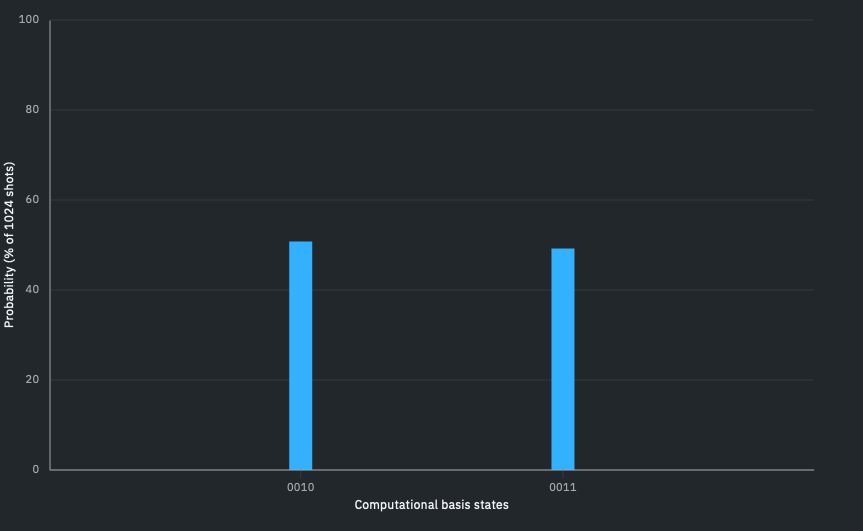
\includegraphics[width=0.66\textwidth]{q3_f_sv.png}
      \captionof{figure}{Screenshot of the results from the IBM Quantum Composer for statevector simulation.}
      \label{fig:3f_sv}
    \end{minipage}

    \begin{minipage}[t]{\textwidth}
      \centering
      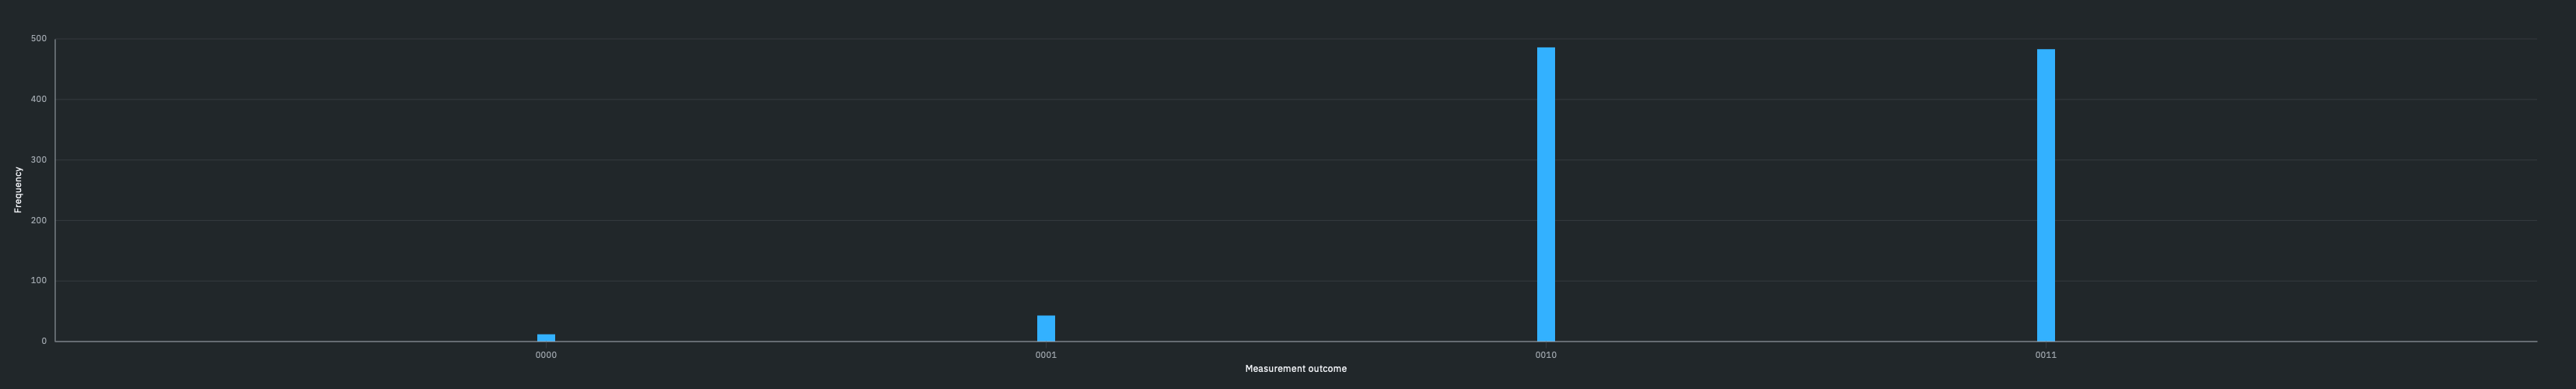
\includegraphics[width=0.9\textwidth]{q3_f_sherbrooke.png}
      \captionof{figure}{Screenshot of the results from the IBM Quantum Composer on IBM Sherbrooke.}
      \label{fig:3f_sb}
    \end{minipage}
    
  \end{proof}
\end{solution}

\begin{solution}[label=ques:3g]
  \begin{question}
    For discrete classical distributions, the Total Variational (TV) distance between two distributions $p$ and $q$ is $\frac{1}{2}\sum_{x \in X} | p(x) - q(x)|$ where $X$ is the set of all possible outcomes. 
Calculate the empirical TV distances of the ideal distribution you calculated in parts (a) to (d) from the distribution produced by the qasm simulator and from the distribution produced by the quantum computer. Show your work.
  \end{question}
  \tcblower{}
  \begin{proof}[Solution]
    The probability distribution for the ideal circuit is $\{0, 0.5, 0, 0.5\}$ for the states $\ket{00}, \ket{01}, \ket{10}, \ket{11}$ respectively. The probability distribution for the statevector simulation is approximately $\{0, 0.507, 0, 0.493\}$. The probability distribution on running it on IBM Sherbrooke is approximately $\{0.011, 0.475, 0.040, 0.474\}$. Note that we consider the states as $\ket{q_0q_1}$, unlike the plots from IBM which consider the states as $\ket{q_1q_0}$. The TV distance between the ideal and statevector simulation is,
    \begin{equation}
      \begin{split}
      \mathsf{TV}(\text{ideal, statevector}) &= \frac{1}{2}\left(|0 - 0| + |0.5 - 0.507| + |0 - 0| + |0.5 - 0.493|\right)\\
      &= \frac{1}{2}(0.007 + 0.007)\\
      &= 0.007
      \end{split}
    \end{equation}
    The TV distance between the ideal and IBM Sherbrooke is,
    \begin{equation}
      \begin{split}
        \mathsf{TV}(\text{ideal, statevector}) &= \frac{1}{2}\left(|0 - 0.011| + |0.5 - 0.475| + |0 - 0.04| + |0.5 - 0.474|\right)\\
        &= \frac{1}{2}(0.011 + 0.025 + 0.04 + 0.026)\\
        &= 0.051
      \end{split}
    \end{equation}
  \end{proof}
\end{solution}
